\documentclass{beamer}
\usepackage[polish]{babel}
\usepackage[utf8]{inputenc}
\usepackage{lmodern}
\usepackage{listings}
\usepackage{graphicx}
\usetheme{AGH}

\lstset{
		language=C++,
		numbers=left,
		columns=fullflexible,
%		frame=single,
  		breaklines=true,
}

\title{Zrównoleglenie algorytmu gradientowej klasteryzacji z użyciem technologii GPU}
\subtitle{Ernest Jęczmionek}
\author{dr hab. inż. Piotr Kowalski}
\institute{Wydział Fizyki i Informatyki Stosowanej}
\date{\today}


\begin{document}

\titleframe[pl]

\begin{frame}\frametitle{Plan prezentacji} %\framesubtitle{...z podtytułem...}
	\tableofcontents
\end{frame}


%----------------------------------------------------------


\section{Cele i narzędzia}
\begin{frame}\frametitle{Cele pracy}
\begin{itemize}
\item implementacja algorytmu w językach C++ oraz CUDA C++ z wykorzystaniem sprzętu konsumenckiego
\item porównanie i analiza wyników
\end{itemize}
\end{frame}

\begin{frame}\frametitle{Narzędzia}
\begin{itemize}
\item C++14 (async), g++ -O3
\item cuda10, cuda capability >= 5.0
\end{itemize}
\end{frame}


%----------------------------------------------------------


\section{Algorytm klasteryzacji gradientowej}
\begin{frame}\frametitle{Schemat algorytmu klasteryzacji gradientowej}
\begin{enumerate}
	\item sformułowanie estymatora jądrowego wraz z jego parametrami
	\item wykonanie przemieszczeń aż do spełnienia warunku zakończenia
	\item procedura tworzenia klastrów
\end{enumerate}
\end{frame}

\begin{frame}\frametitle{Estymator jądrowy}
\begin{center}
$\hat{f}(x)=\frac{1}{mh^n} \displaystyle \sum_{i=1}^{m} \frac{1}{s_i}K(\frac{x-x_i}{hs_i})$ \\~\
gdzie $h = min(g(h))$ \\~\
$g(h)=\frac{1}{m^2h^2}\displaystyle\sum_{i=1}^{m} \displaystyle\sum_{j=1}^{m} \widetilde{K}(\frac{x_j - x_i}{h}) + \frac{2}{mh^n}K(0)$ \\~\
$s_i = {\frac{\hat{f}_*(x_i)}{\bar{s}}}^{-c}$ \\~\
\end{center}
\end{frame}

\begin{frame}\frametitle{Warunek zakończenia}
\begin{center}
$x_j^{k+1} = x_j^k + b\frac{\nabla f(x_j^k)}{f(x_j^k)}$ \\~\
dopóki $|D_k - D_{k-1}| \leq \alpha D_0$ \\~\
gdzie $D_k = \displaystyle\sum_{i=1}^{m-1} \displaystyle\sum_{j=i+1}^{m} d(x_i^k, x_j^k)$
\end{center}
\end{frame}

\begin{frame}\frametitle{Wyznaczenie odległości międzyklastrowej}
\begin{center}
należy wyznaczyć zbiór wszytkich odległości między elementami \\~\
$\{d(x^{k*}_i, x^{k*}_j)_{i \neq j}\}$ \\~\
oraz znaleźć najmniejszy element zbioru \\~\
$\{0.01 \sigma_d, 0.02 \sigma_d, ... , int(100D-1) 0.01 \sigma_d \}$ \\~\
spełniający warunek \\~\
$\hat{f}_d(x-0.01\sigma_d) > \hat{f}_d \wedge \hat{f}_d \leq \hat{f}_d(x+0.01\sigma_d)$
\end{center}
\end{frame}

\begin{frame}\frametitle{Procedura tworzenia klastrów}
\begin{enumerate}
\item pobierz element zbioru i utwórz z niego jednoelementowy klaster
\item znajdź inny element w odległości $x_d$ i dodaj go do klastru, gdy jest to niemożliwe przejdź do Punktu 4
\item znajdź inny element w odległości $x_d$ od dowolnego elementu klastru i dodaj go oraz powtórz Punkt 3
\item zaakceptuj utworzony klaster i usuń ze zbioru jego elementy, gdy zbiór nie jest pusty powróć do Punktu 1
\end{enumerate}
\end{frame}


%----------------------------------------------------------


\section{Implementacja}
\begin{frame}\frametitle{Zrównoleglenie CPU}
\lstinputlisting[language=C++, firstline=1, lastline=15, basicstyle=\small]{code.cpp}
\end{frame}

\begin{frame}\frametitle{Zrównoleglenie GPU}
\lstinputlisting[language=C++, firstline=20, lastline=28, basicstyle=\small]{code.cpp}
\end{frame}

\begin{frame}\frametitle{Zrównoleglone fragmenty algorytmu }
\begin{itemize}
\item estymator jądrowy - $\hat{f}$, $s_i$
\item funkcja $g(h)$
\item funkcje odległości $D_k$
\end{itemize}
\end{frame}

\begin{frame}\frametitle{Procedura tworzenia klastrów}
\begin{center}
Niniejszy fragment algorytmu jest sekwencyjny!
\end{center}
\end{frame}


%----------------------------------------------------------


\section{Wyniki}
\begin{frame}\frametitle{Wyniki wydajnościowe}
\begin{table}[]
\resizebox{\textwidth}{!}{%
\begin{tabular}{|c|c|c|c|c|c|c|c|}
\hline
Unit \textbackslash data size                                           & 10    & 50    & 100   & 150   & 250    & 400   & 1000 \\ \hline
\begin{tabular}[c]{@{}c@{}}i7 4710HQ\\ (4 cores)\end{tabular}           & 131ms & 2.6s  & 51s   & 4m7s  &        &       &      \\ \hline
\begin{tabular}[c]{@{}c@{}}i7 7700HQ \\ (4 cores)\end{tabular}          & 112ms & 2.9s  & 40s   & 3m22s & 26m55s &       &      \\ \hline
\begin{tabular}[c]{@{}c@{}}GTX 850m \\ (640 cuda cores)\end{tabular}    & 121ms & 0.22s & 1.25s & 5.69s & 45s    & 5m30s &      \\ \hline
\begin{tabular}[c]{@{}c@{}}GTX 1070m \\ (2048 cuda cores)\end{tabular} & 439ms & 0.19s & 0.41s & 4.86s & 57s    & 4m30s & 71m  \\ \hline
\end{tabular}%
}
\end{table}
\end{frame}

\begin{frame}\frametitle{Profiler GPU}
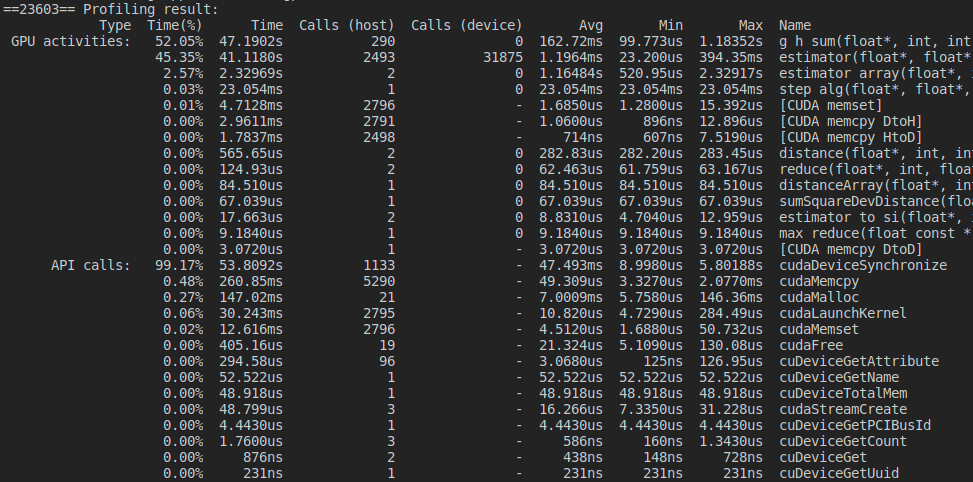
\includegraphics[width=\textwidth]{nvprof250}
\end{frame}

\begin{frame}\frametitle{Wyniki jakościowe}
\begin{itemize}
\item występują rozbieżności w obliczeniach dla większych ilości danych, prawdopodobnie jest to spowodowane niedostateczną precyzją obliczeń typu float(32bit)
\item niektóre zbiory danych powodują wyznaczenie różnych parametrów wygładzania, co wpływa na wyznaczenie odległości międzyklastrowej
\end{itemize}
\end{frame}

\begin{frame}\frametitle{Wnioski}
\begin{itemize}
\item algorytm nie zachowuję się stabilnie dla typu float(32bit), a karty graficzne posiadające jednostki FP64 nie leżą w obszarze konsumenckim
\item użycie algorytmu na klastrze, będzie wiązało się z kopiowaniem wszystkich danych oraz ich synchronizacją co w praktyce nie wniesie wkładu wydajnościowego
\end{itemize}
\end{frame}

%----------------------------------------------------------

\begin{frame} \frametitle{Źródła}
\begin{thebibliography}{10}
\beamertemplatearticlebibitems
  \bibitem{Autor1990}
    P.~Kulczycki A.~Charatynowicz
    \newblock {\em A complete gradient clustering algorithm formed with kernel estimators}.
    \newblock International Journal of Applied Mathematics and Computer Science, vol. 20, nr 1, ss. 123-134, 2010
  \beamertemplatearticlebibitems
  \bibitem{Jemand2000}
    M.~Harris.
    \newblock Optimizing Parallel Reduction in CUDA
    \newblock {\em Robot Intelligence Technology Lab. 2016}
\end{thebibliography}
\end{frame}

\begin{frame}
\begin{center}
\Huge Dziękuję za uwagę
\end{center}
\end{frame}


\end{document}
